\documentclass[11pt]{article}

\usepackage[utf8]{inputenc}
\usepackage[T1]{fontenc}
\usepackage{lmodern}
\usepackage[margin=1in]{geometry}
\usepackage{graphicx}
\usepackage{amsmath}
\usepackage{booktabs}
\usepackage{microtype}
\usepackage{siunitx}
\usepackage{xcolor}
\usepackage[hidelinks]{hyperref}
\usepackage[numbers,sort&compress]{natbib}
\usepackage{caption}
\captionsetup{font=small,labelfont=bf}

\newcommand{\fps}{\textsc{fps}}
\newcommand{\celegans}{\textit{C.\ elegans}}

\title{\textbf{What Survives Compression and What Does Not:\\
An In-Silico Audit of Connectome-Based Mind-Migration Proposals\\
Using a Functional Preservation Score}}
\author{[Author(s) withheld for review]}
\date{Preprint --- \today}

\begin{document}
\maketitle

\begin{abstract}
\noindent
Speculative proposals for ``mind migration'' describe reading a brain's identity, compressing it,
and installing it into a new substrate. Such proposals assemble several active research areas
(connectomics, graph neural networks, memory prosthetics, neural interfaces, optogenetics) into a
single pipeline, typically relying on the most optimistic reading of each. We examine the
computational core of this pipeline directly, using an auditable procedure on public data that
runs on a single laptop. The study is organised around a Functional Preservation Score (\fps):
a null-normalised, behaviourally grounded measure of how much of a neural system's input--output
function survives an operation such as compression, alignment, transport, or writing. We apply
\fps\ across five pre-registered studies on the \celegans\ connectome, whole-brain calcium
activity~\citep{kato2015global}, and hippocampal replay (DANDI~000044).

Two of the studies yield positive characterisations and three form a negative result. First,
low-bit quantisation of a real connectome runs into a structure-dependent sparsity floor: uniform
int4/ternary quantisation is forced to roughly $73\%/98\%$ effective sparsity because the
heavy-tailed integer synaptic weights round to zero, whereas mixed-precision protection of hub
neurons lowers these floors to about $27\%/32\%$. Second, decoded hippocampal replay sequences
compress heavily while remaining identifiable: a 48-unit $\times$ 25-bin sequence ($\sim$38~kbit)
stays identifiable at a cross-validated top-1 accuracy of $0.69$ (95\% CI $[0.63,0.74]$; chance
$0.125$; permutation $p<10^{-3}$) from latents on the order of $10$--$50$ bits per event, and a
bounded ``background-sync'' store shows a graceful-versus-cliff trade-off between capacity and
interference. Third, the migration pipeline fails in simulation at each stage, for largely
independent reasons. The putative ``identity payload'' is not a functionally separable module
(permutation $p\geq0.16$ at every tested size). Cross-individual functional transport collapses
once the target's actual wiring is respected (fidelity $1.00\!\to\!0.40$, 95\% CI $[0.31,0.49]$,
$p<10^{-3}$) or the alignment is imperfect ($0.06$, $[0.00,0.13]$). And the proposed biologically
plausible write mechanism cannot reach the function the target topology provably admits
(plausibility gap $0.45$, 95\% CI $[0.27,0.64]$, $p<10^{-3}$, $d=2.0$).

Taken together, compression of neural data is a quantifiable phenomenon, while migration of
function across substrates is not supported by the proposed pipeline on the systems we can
currently test. We release \fps, the dataset loaders, and the full set of operations as a
measurement toolkit.

\medskip
\noindent\textbf{Scope.} All results are obtained on a 306-neuron nematode connectome, small
recurrent networks, and reflex- or trajectory-scale functions. They say nothing about reading or
writing a living human brain. The biological prerequisites for the full pipeline remain absent,
and we make no claim about them; the studies test coherence in simulation, not biological
feasibility.
\end{abstract}

\section{Introduction}
A recurring theme in recent discussions of biological aging is to treat it as a reversible
information-processing problem. Mind migration is one speculative endpoint of that view. In the
version we examine, a brain is partitioned into a regenerable ``Base-OS'' (autonomic, sensory, and
motor circuitry) and a transferable ``identity payload'' (association cortex and hippocampus);
the payload is then compressed through sparsification and low-bit quantisation, aligned to a
differently wired target brain, and installed through activity-dependent plasticity. Each of
these steps draws on a real experimental result, but the composition has never been tested as a
whole, and several of the links have no supporting evidence at any scale.

We do not attempt the biological pipeline, which is infeasible with current or foreseeable tools.
Instead we treat preservation of function as a measurable quantity and ask which stages of the
computational pipeline can actually be built, and where and why the remaining ones fail. Posing
the question this way turns an otherwise unfalsifiable goal into a measurement problem that admits
decision-relevant evidence from public data on ordinary hardware.

The paper makes five contributions. (1)~We define \fps, a substrate-agnostic measure of functional
preservation with an explicit trivial-baseline null (\S\ref{sec:fps}). (2)~We characterise
compression of a real connectome and identify a quantisation sparsity floor (\S\ref{sec:t1}).
(3)~We characterise the compressibility of real hippocampal replay sequences and describe a
capacity--interference relationship for bounded storage (\S\ref{sec:t3}). (4)~We provide a
three-stage in-silico test of the partition--align--write pipeline and locate the failure mode at
each stage (\S\ref{sec:t3stages}). (5)~We release a reproducible, laptop-scale toolkit
(\S\ref{sec:repro}).

\section{Related work and claim provenance}
We checked the frontier results that the pipeline depends on against their primary sources. Most
are genuine, but several are mis-attributed or overstated in popular accounts. On synaptic
turnover and memory, torpor is known to shed roughly 50--65\% of synapses with memory
preserved~\citep{vonderohe2006torpor}, which supports sparsification that is structured rather
than uniform. On connectome-driven models, FlyWire~\citep{dorkenwald2024flywire} and
flyGNN~\citep{flygnn2025} show that a connectome can drive simulated behaviour, but only once the
dynamical parameters are fitted; the topology alone does not suffice. On memory prosthetics, the
multi-input multi-output devices of \citet{hampson2018prosthetic} improved human recall by about
35--37\%, but this is restoration within a single subject rather than transfer of identity between
subjects. On neural interfaces, high-density wireless arrays~\citep{jung2025bisc} record from the
subdural surface and do not read at synaptic resolution. On alignment, Gromov--Wasserstein optimal
transport aligns brains at the scale of functional parcels~\citep{thual2022fugw,xu2019gwl}, but it
is NP-hard and has not been tested for functional transport on connectomes.

Generic graph-network pruning and quantisation~\citep{gnnprunequant2025} and scalable
Gromov--Wasserstein~\citep{xu2019sgwl} are established methods. What is new here is their
composition on connectome substrates under a functional, behaviourally grounded metric, together
with the explicit test of the migration stages that have no empirical basis.

\section{Methods}

\subsection{Functional Preservation Score}\label{sec:fps}
Let a system map a fixed battery of stimuli to outputs. For a reference system with outputs
$Y_{\mathrm{ref}}$ and a transformed system with outputs $Y$, define an $R^2$-style fit
$\mathrm{raw}(Y)=1-\lVert Y-Y_{\mathrm{ref}}\rVert^2/\lVert Y_{\mathrm{ref}}-\overline{Y_{\mathrm{ref}}}\rVert^2$.
The score is normalised by the best trivial baseline, the larger of a shuffled stimulus--response
mapping and a predict-the-mean baseline:
\begin{equation}
\fps = \mathrm{clip}\!\left(\frac{\mathrm{raw}(Y)-\mathrm{raw}(Y_{\mathrm{null}})}{1-\mathrm{raw}(Y_{\mathrm{null}})},\,0,\,1\right).
\end{equation}
An \fps\ of 1 means the transformed system reproduces the reference function; an \fps\ of 0 means
it performs no better than the best trivial control. Normalising by the null matters in practice,
because without it a system that always produces a plausible-looking but input-independent output
can score deceptively well. For identity-style tasks we also use identification accuracy, which
asks whether reconstruction $i$ is nearest to its own original among all events; it is bounded and
has an exact chance level $1/n$.

\subsection{Substrates and data}
We use the White/Cook \celegans\ somatic connectome~\citep{white1986structure,cook2019connectome}
via the OpenWorm ConnectomeToolbox (306 neurons, 3{,}158 edges; 81 sensory, 95 interneuron, 130
motor). Dynamics are a leaky-rate $\tanh$ recurrent model reading out motor neurons over a fixed
low-pass stimulus battery. Whole-brain calcium activity is from \citet{kato2015global} (5 worms,
$\sim$109--135 neurons). Hippocampal replay is from DANDI~000044~\citep{grosmark2016diversity,diba2007forward}
(Buddy session, 48 pyramidal units plus linearised position, streamed without full download), with
a nelpy CA1 linear-track session for the structure gate.

\subsection{Operations and statistics}\label{sec:stats}
Compression uses magnitude pruning (uniform) versus engram-aware pruning that protects
high-degree, betweenness, or $k$-core hubs, with symmetric quantisation to int8/int4/ternary and
an optional mixed precision that keeps hubs at higher bit depth; policies are compared at matched
total effective sparsity. Alignment uses a self-contained entropic Gromov--Wasserstein solver
(square loss with Sinkhorn projection~\citep{peyre2016gw}); transport pushes weights through a
node correspondence under a Peters'-rule feasibility mask. The write stage uses a fixed-topology
rate host with strictly local three-factor plasticity (audited: no backprop, no per-weight target
gradient) and a global least-squares optimiser as an upper bound.

All headline numbers are reported as a point estimate with a percentile bootstrap 95\% confidence
interval (10{,}000 resamples) over the relevant randomisation, with the sample size stated.
Comparisons carry a one-sided permutation test (10{,}000 permutations, add-one-corrected) and,
where applicable, Cohen's $d$. To avoid selection bias we report a pre-registered primary engram
policy (strength) rather than the maximum over variants. The identification frontier uses 30-split
repeated cross-validation with the autoencoder fit on the training split only.

\section{Study 1: Connectome compression}\label{sec:t1}
We ask how far a connectome-driven model can be compressed, along sparsity, bit depth, and
structure, before its function collapses, and whether structured sparsification outperforms
uniform pruning. At matched effective sparsity under int4, using the pre-registered primary policy
and eight stimulus seeds, the engram-aware policy preserves function better than uniform pruning:
\fps\ of $0.30$ (95\% CI $[0.12,0.48]$) versus $0.03$ ($[0.00,0.09]$) at target sparsity 0.5
($p=0.015$, $d=1.3$), with comparable margins at 0.6 and 0.7.

The central finding is the floor (Fig.~\ref{fig:t1}). Uniform quantisation cannot reach low
sparsity on the real connectome, because the heavy-tailed integer weights round to zero: the
effective-sparsity floor is $0.73$ for int4 and $0.98$ for ternary under uniform quantisation,
against $0.27$ and $0.32$ under engram-aware mixed precision. At int8 there is no floor. These
floors are deterministic properties of the weight distribution. The structured advantage, by
contrast, is not robust: in a clean int8 comparison it depends on regime and does not reproduce
under an independent sigmoid-conductance model, so we drop the broader claim and retain only the
floor.

\begin{figure}[t]
\centering
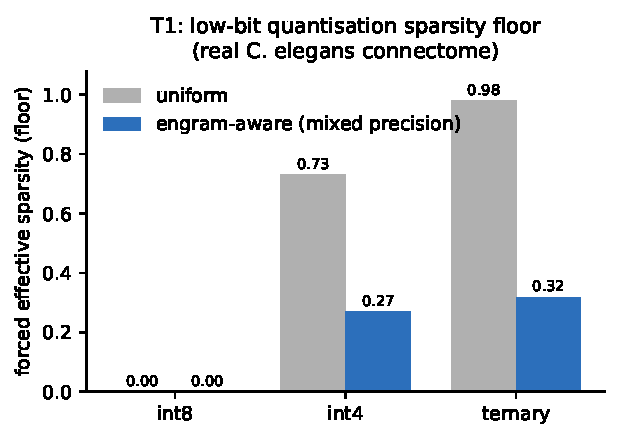
\includegraphics[width=0.52\linewidth]{figures/fig1_t1_floor.pdf}
\caption{Low-bit quantisation imposes an effective-sparsity floor on the real \celegans\
connectome under uniform quantisation (grey); mixed-precision hub protection (blue) lowers it.
The floors are deterministic weight-distribution properties.}
\label{fig:t1}
\end{figure}

\section{Study 2: Replay-sequence compression}\label{sec:t3}
We ask whether decoded hippocampal replay sequences can be compressed to few bits while preserving
their content. Place-ordered run-epoch sequences first show decodable trajectory structure
(Bayesian decode score $0.34$ versus a time-shuffled null of $0.20$ across 62 sequences). Under
30-split cross-validation with the autoencoder fit on the training split only, the uncompressed
model identifies held-out replay events at top-1 $0.69$ (95\% CI $[0.63,0.74]$) against chance
$0.125$ (permutation $p=10^{-4}$). Identification degrades gradually with the bit budget, with
non-overlapping intervals, so a 48$\times$25 sequence ($\sim$38~kbit raw) remains well above chance
down to roughly 8--16 bits per event, a compression ratio of order $10^3$ (Fig.~\ref{fig:t3}, left).
Streaming events into a fixed-size store (Fig.~\ref{fig:t3}, right) shows a genuine capacity limit:
a superposition store degrades gradually while a slot store is perfect to capacity and then drops
sharply. These results make the compressed-backup idea plausible as compression of decoded
sequences; they do not show that such a backup contains a memory.

\begin{figure}[t]
\centering
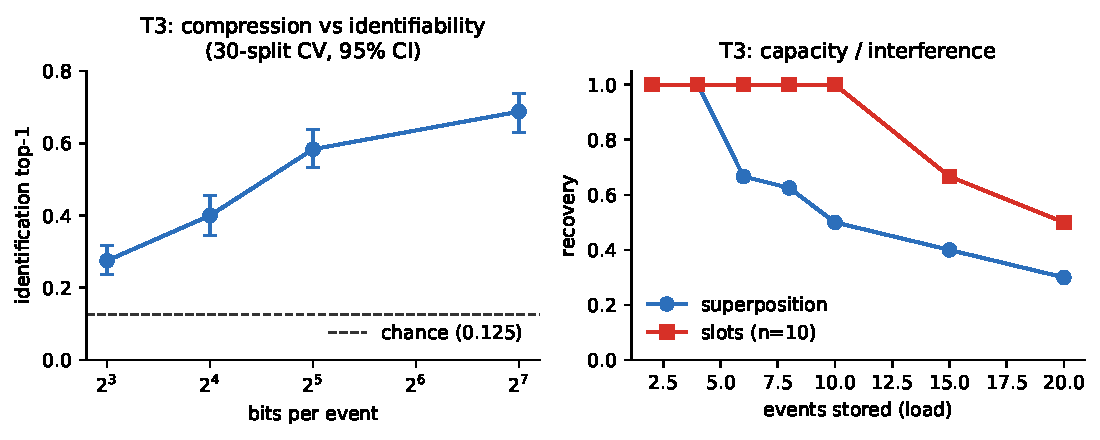
\includegraphics[width=0.92\linewidth]{figures/fig2_t3_frontier.pdf}
\caption{Left: identification accuracy versus latent bit budget under 30-split cross-validation
(95\% CI); dashed line is chance. Right: recovery from a fixed-size incremental store versus load,
for a superposition store and a slot store.}
\label{fig:t3}
\end{figure}

\section{Study 3: The migration pipeline in simulation}\label{sec:t3stages}
Each stage is a surrogate test of a biological stage for which no direct evidence exists; the
question is whether the stage is coherent in simulation on the nearest testable substrate.

\paragraph{Partition separability.} Holding the sensory and motor interface fixed, we test whether
ablating the asserted interneuron payload degrades the input--output transformation more than
ablating a random interneuron subset of the same size. It does not. Against a 500-sample null, the
asserted payload is not significantly more disruptive at any tested size (permutation $p=0.17,
0.16, 0.27, 0.37$ at payload fractions $0.1$--$0.4$). We find no significantly separable identity
module; the function is distributed.

\paragraph{Functional transport.} With a second individual generated as a controlled-divergence
perturbation of the first, entropic Gromov--Wasserstein recovers $0.76$ (95\% CI $[0.74,0.78]$) of
the ground-truth correspondence at 5\% rewiring. The transport, however, does not survive
realistic conditions (Fig.~\ref{fig:t2}). Given an oracle correspondence and unconstrained
writing, fidelity is $1.00$; once the transported weights must respect the target's wiring, it
falls to $0.40$ (95\% CI $[0.31,0.49]$, $p=3\times10^{-4}$); using the estimated correspondence it
is $0.06$ ($[0.00,0.13]$, $p=2\times10^{-4}$). High correspondence accuracy does not imply
preserved function; the binding constraint is the target's own wiring.

\paragraph{Local-rule writing.} Across ten seeds, a global optimiser reaches a ceiling of $1.00$,
confirming the topology can host the function, while strictly local reward-modulated plasticity
reaches only $0.55$ (95\% CI $[0.36,0.73]$), leaving a plausibility gap of $0.45$ ($[0.27,0.64]$,
$p=10^{-4}$, $d=2.0$; Fig.~\ref{fig:t4}). Ripple-timed gating confers no advantage (the
ripple-minus-continuous difference has a CI including zero).

\begin{figure}[t]
\centering
\begin{minipage}{0.48\linewidth}
\centering
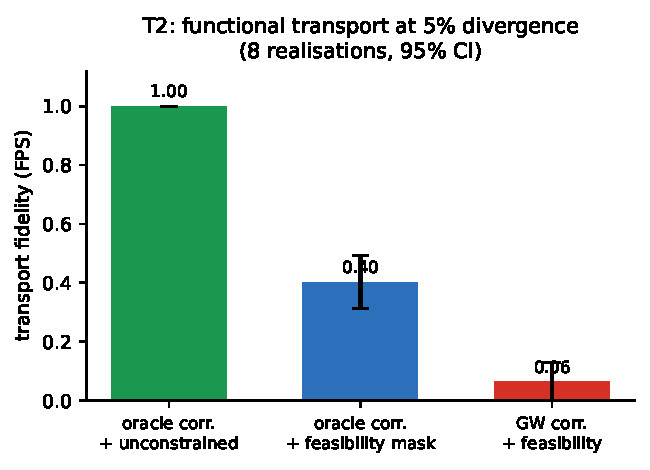
\includegraphics[width=\linewidth]{figures/fig3_t2_transport.pdf}
\caption{Transport fidelity at 5\% divergence. The feasibility mask and imperfect alignment each
collapse fidelity relative to the oracle/unconstrained ideal.}
\label{fig:t2}
\end{minipage}\hfill
\begin{minipage}{0.46\linewidth}
\centering
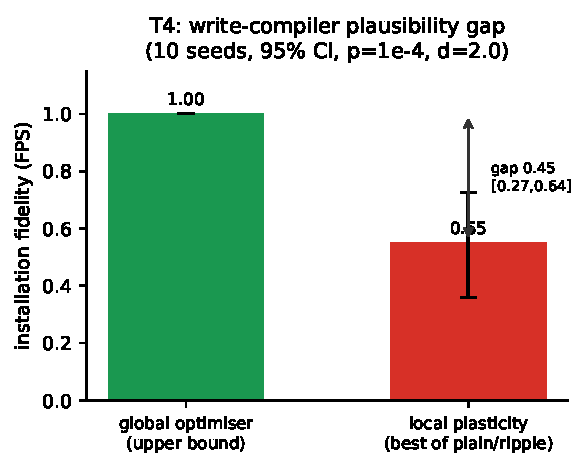
\includegraphics[width=\linewidth]{figures/fig4_t4_gap.pdf}
\caption{The write-compiler plausibility gap: a global optimiser succeeds where local plasticity
does not, on the same feasible topology.}
\label{fig:t4}
\end{minipage}
\end{figure}

\paragraph{The three stages together.} The stages fail for largely independent, compounding
reasons: there is no clean module to extract; even the whole graph cannot be placed once alignment
is imperfect and the target's wiring is respected; and even where the topology can host the
function, the proposed write mechanism cannot reach it. The target substrate's own wiring is the
limit common to the last two stages.

\section{Discussion}
The computational core of the pipeline separates into two parts. Compression of neural data is
measurable and bounded (Studies 1 and 2). Migration of function across substrates is not supported
by the proposed partition--align--write pipeline (Study 3), with the target substrate's wiring as
the recurring obstacle. Several limitations qualify these conclusions. The work is at small scale
(a 306-neuron connectome, activity recordings of at most 135 neurons, and 40-neuron networks);
the dynamics are simple rate models; some test sets are small; the second individual in Study 2 is
a divergence model of a single real connectome; and \fps\ is a functional measure, not a claim
about subjective experience. The biological prerequisites for the full pipeline remain absent and
are not addressed. All work is computational on public animal datasets, with no human subjects,
wet-lab, organoid, or cloning work.

\section{Reproducibility}\label{sec:repro}
All results are deterministic and run on a laptop. Each claim maps to a committed JSON artifact and
the script that produced it. Data are fetched via documented scripts; the metric, loaders, and
operations are released, and a test suite covers the substrate contracts. Statistically hardened
artifacts (bootstrap CIs and permutation $p$-values) accompany each headline claim.

\section*{Acknowledgements}
We thank the OpenWorm, FlyWire, and DANDI communities for public data.

\bibliographystyle{plainnat}
\bibliography{references}

\end{document}
